\lstset {
	numbers=none,
	frame=none
}
\setcounter{figure}{0}
\section{Guía de puesta en marcha}
En esta anexo se explicará paso a paso como poner en marcha el sistema. Se asume que el lector de esta guía tiene conocimientos básicos de manejo de bash en GNU/Linux.

Para proceder se necesitan los siguientes elementos:
\begin{itemize}
	\item PC corriendo Debian 9 \enquote{Stretch} con ambiente de escritorio GNOME. No es necesario que sea precisamente esta distribución de GNU/Linux pero esta guía explicara los pasos para esta distribución en particular.
	\item Un módulo maestro.
	\item Al menos un modulo esclavo.
	\item Cable Micro-USB.
	% Herramientas?
\end{itemize}

\subsection{Compilación del firmware}\label{sec:comp-firmware}
En esta sección se explicará como instalar el kit de desarrollo de software de Espressif y cómo cargar el firmware al SoC (System on Chip). Para esto es necesario instalar software para traer el repositorio git y compilar el compilador que se utilizará. El compilador es el gcc de GNU pero modificado para generar código para el procesador Tonsillica Xtensa LX106, que es el que utiliza el ESP8266EX.

\subsubsection{Compilación del toolchain}
Los comandos que comiencen con \enquote{\#} deben hacerse siendo el superusuario. Una manera de abrir una sesión es usar el comando \code{su}, que permite iniciar una sesión de bash como root, el superusuario del sistema.

Primero hay que descargar \code{git} para poder clonar repositorio (este paso también aplica para la aplicación de pc):
\begin{lstlisting}
# apt install git -y
\end{lstlisting}
Debería aparecer texto similar al siguiente:
\begin{lstlisting}
root@tpi:/home/ramiro# apt install git -y
Leyendo lista de paquetes... Hecho
Creando árbol de dependencias       
Leyendo la información de estado... Hecho
Paquetes sugeridos:
  git-daemon-run | git-daemon-sysvinit git-doc git-el git-email git-gui gitk
  gitweb git-arch git-cvs git-mediawiki git-svn
Se instalarán los siguientes paquetes NUEVOS:
  git
0 actualizados, 1 nuevos se instalarán, 0 para eliminar y 0 no actualizados.
Se necesita descargar 4.160 kB de archivos.
Se utilizarán 29,5 MB de espacio de disco adicional después de esta operación.
Des:1 http://ftp.ccc.uba.ar/pub/linux/debian/debian stretch/main amd64 git amd64 1:2.11.0-3+deb9u2 [4.160 kB]
Descargados 4.160 kB en 1s (2.162 kB/s)
Seleccionando el paquete git previamente no seleccionado.
(Leyendo la base de datos ... 148278 ficheros o directorios instalados actualmente.)
Preparando para desempaquetar .../git_1%3a2.11.0-3+deb9u2_amd64.deb ...
Desempaquetando git (1:2.11.0-3+deb9u2) ...
Configurando git (1:2.11.0-3+deb9u2) ...
\end{lstlisting}

Luego, hay que descargar el SDK NON-OS para poder generar el firmware. Existe un repositorio github con un ambiente prearmado, ya que la alternativa propuesta por Espressif es descargar una imagen de una máquina virtual con Ubuntu y las herramientas ya configuradas.

Estando en el directorio home del usuario, ejecute los siguientes comandos en secuencia:
\begin{lstlisting}
$ cd
$ git clone --recursive https://github.com/pfalcon/esp-open-sdk
$ cd esp-open-sdk
\end{lstlisting}

El paso de \code{git clone} debería producir la siguiente salida:
\begin{lstlisting}
ramiro@tpi:~$ git clone --recursive https://github.com/pfalcon/esp-open-sdk
Cloning into 'esp-open-sdk'...
remote: Counting objects: 539, done.
remote: Total 539 (delta 0), reused 0 (delta 0), pack-reused 539
Receiving objects: 100% (539/539), 335.47 KiB | 296.00 KiB/s, done.
Resolving deltas: 100% (311/311), done.
Submodule 'crosstool-NG' (https://github.com/jcmvbkbc/crosstool-NG) registered for path 'crosstool-NG'
Submodule 'esp-open-lwip' (https://github.com/pfalcon/esp-open-lwip) registered for path 'esp-open-lwip'
Submodule 'esptool' (https://github.com/themadinventor/esptool) registered for path 'esptool'
Submodule 'lx106-hal' (https://github.com/tommie/lx106-hal) registered for path 'lx106-hal'
Cloning into '/home/ramiro/esp-open-sdk/crosstool-NG'...
remote: Counting objects: 33801, done.        
remote: Total 33801 (delta 0), reused 0 (delta 0), pack-reused 33800        
Receiving objects: 100% (33801/33801), 17.06 MiB | 2.39 MiB/s, done.
Resolving deltas: 100% (20003/20003), done.
Cloning into '/home/ramiro/esp-open-sdk/esp-open-lwip'...
remote: Counting objects: 236, done.        
remote: Total 236 (delta 0), reused 0 (delta 0), pack-reused 236        
Receiving objects: 100% (236/236), 495.14 KiB | 317.00 KiB/s, done.
Resolving deltas: 100% (75/75), done.
Cloning into '/home/ramiro/esp-open-sdk/esptool'...
remote: Counting objects: 1466, done.        
remote: Total 1466 (delta 0), reused 0 (delta 0), pack-reused 1466        
Receiving objects: 100% (1466/1466), 4.97 MiB | 1.29 MiB/s, done.
Resolving deltas: 100% (890/890), done.
Cloning into '/home/ramiro/esp-open-sdk/lx106-hal'...
remote: Counting objects: 122, done.        
remote: Total 122 (delta 0), reused 0 (delta 0), pack-reused 122        
Receiving objects: 100% (122/122), 179.61 KiB | 0 bytes/s, done.
Resolving deltas: 100% (51/51), done.
Submodule path 'crosstool-NG': checked out '37b07f6fbea2e5d23434f7e91614528f839db056'
Submodule path 'esp-open-lwip': checked out '8c39d2179a273553466043f388772abb6251a4ca'
Submodule path 'esptool': checked out '9dfcb350e1a91bb4641f725fc6c2f126791013ce'
Submodule path 'lx106-hal': checked out 'e4bcc63c9c016e4f8848e7e8f512438ca857531d'
\end{lstlisting}

Ahora se necesitan instalar dependencias propias del repositorio recién descargado para poder compilar las herramientas de desarrollo. Con el siguiente comando se descargarán todos los paquetes necesarios:
\begin{lstlisting}
# apt install make unrar-free autoconf automake libtool gcc g++ gperf flex bison texinfo gawk ncurses-dev libexpat-dev python-dev python python-serial sed git unzip bash help2man wget bzip2 libtool-bin -y
\end{lstlisting}

Este paso puede tardar mucho o poco dependiendo de la velocidad de la conexión a Internet.

Una vez descargados todos los componentes, ingrese el siguiente comando para iniciar la compilación de las herramientas, asegurandose de {\bfseries no} ser el superusuario:

\begin{lstlisting}
$ make standalone=n
\end{lstlisting}

El makefile de este repositorio ofrece dos alternativas al momento de compilar las herramientas: si se utiliza \code{standalone=y} entonces las cabezeras y archivos objetos privativos de Espressif se acoplan al compilador, lo cual hace que no sea necesario especificar al linkeador las librerías a las cuales hay que linkear. Sin embargo, esta alternativa hace dificil personalizar algunos aspectos del linkeo y, cómo se verá mas adelante, este proyecto necesita reemplazar unas de las librerías del SDK, con lo cual se utiliza en este caso \code{standalone=n}.

Este paso toma desde 30 minutos a 2 horas, dependiendo de las prestaciones de la computadora utilizada. Al terminar debe aparecer el siguiente mensaje:

\begin{lstlisting}
Espressif ESP8266 SDK is installed, its libraries and headers are merged with the toolchain
\end{lstlisting}


Una vez terminada la compilación, hay que realizar un paso que soluciona un problema en el que el software del cartel falla en la etapa de linkeo por no entrar en una RAM dedicada a instrucciones que utiliza el ESP8266EX. Lamentablemente no hay mucha información disponible de por qué pasa esto. Como se menciono anteriormente, el SDK es privativo y no muy bien documentado, con lo que la información que circula en Internet es un mejor caso especulativa. Este paso consiste en mover un archivo (específicamente, la implementación de la libreria estándar de C) del directorio del SDK al directorio del compilador.

Estando en el directorio \code{esp-open-sdk}, ingrese el siguiente comando:
\begin{lstlisting}
	cp sdk/lib/libgcc.a xtensa-lx106-elf/lib/gcc/xtensa-lx106-elf/4.8.5/
\end{lstlisting}

Ahora hay que dejar el compilador y las librerías en un lugar fijo, para poder invocar a los comandos y que el código linkee correctamente.

Estando en el directorio \code{esp-open-sdk}, ingrese los siguientes comandos como root:
\begin{lstlisting}
# mkdir /opt/espressif
# mv ESP8266_NONOS_SDK_V2.0.0_16_08_10 /opt/espressif/sdk
# mv xtensa-lx106-elf/ /opt/
# touch /opt/espressif/sdk/include/user_config.h
# echo "PATH=/usr/local/sbin:/usr/local/bin:/usr/sbin:/usr/bin:/sbin:/bin:/opt/xtensa-lx106-elf/bin" >> /etc/profile
# echo "export PATH" >> /etc/profile
\end{lstlisting}

Los últimos dos pasos se encargan de que los paths de los directorios donde se encuentran las herramientas ejecutables (compilador, linkeador, etc) estén en la variable de entorno PATH. Esto es necesario para poder invocar al compiladr estando en cualquier directorio sin tener que referenciarlo con su path entero.

Reinicie la PC o máquina virtual para que los últimos cambios tomen efecto.

\subsubsection{Cambio de librería de TLS}
El módulo que implementa las conexiones TLS en el ESP8266EX tiene unos problemas de implementación que provocan que el microcontrolador se congele por completo. Este problema es reconocido por Espressif y su solución consiste en aplicar un parche al SDK que reemplaza esa librería por una alternativa.

Para descargar el parche ingrese:
\begin{lstlisting}
$ cd
$ wget http://espressif.com/sites/default/files/sdks/esp8266_nonos_sdk_mbedtls_20160718.zip
$ unzip esp8266_nonos_sdk_mbedtls_20160718.zip
\end{lstlisting}

Luego, como root:

\begin{lstlisting}
# cp -rf ESP8266_NONOS_SDK_MBEDTLS/lib /opt/espressif/sdk/
\end{lstlisting}


\subsection{Generación de certificados TLS}\label{sec:cert-gen}
Como se explicó en la sección \ref{sec:tls}, la dirección de IP que toma el dispositivo está asociada al certificado público que exhibe y por lo tanto debe ser estática. En esta sección se explicarán los pasos para, una vez decidida una dirección IP para el cartel, generar el certificado con la clave pública, además de la clave privada.

El SDK provee un script que genera automáticamente el certificado y la clave privada. La clave privada y el certificado se almacenarán en el firmware del cartel y el certificado se almacenará en el ejecutable de la aplicación de PC. Esto es porque, normalmente, los certificados están firmados electrónicamente por una \enquote{Certificate Authority} o CA. En este caso el certificado de este proyecto se denomina \emph{self-signed}, con lo que es necesario \enquote{notificar} a la aplicación de PC que ese certificado es confiable.

En el directorio \code{/opt/espressif/sdk/tools} hay un archivo \code{makefile.sh}. Este es el script que generará el certificado y clave primaria. Hay que modificar el contenido de \code{makefile.sh} para definir la IP que utilizará el cartel.

Ingrese el siguiente comando para realizar una copia de seguridad del script:
\begin{lstlisting}
$ cp makefile.sh makefile.sh.bak
\end{lstlisting}

Y luego, edite \code{makefile.sh} tomando como guía la figura \ref{fig:guia-cert}.

\begin{figure}[!hbpt]
	\centering
	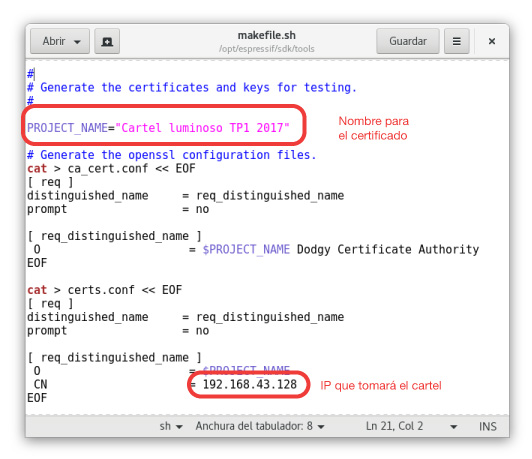
\includegraphics[height=10cm]{imagenes/cert-screenshot.jpg}
	\caption{El archivo \code{makefile.sh} con los datos que hay cambiar señalados.}
	\label{fig:guia-cert}
\end{figure}

Hecho esto, ejecute:

\begin{lstlisting}
$ chmod +x makefile.sh
$ ./makefile.sh
\end{lstlisting}

Esto produce el certificado y clave privada en distintos formatos. Para el sistema solo se necesitan \code{private\_key.h}, \code{cert.h} y \code{TLS.ca\_x509.cer}. Los primeros dos se utilizan en el firmware del cartel y el último es para la aplicación de PC, con lo que no debe eliminarse ya que se utilizará mas adelante en esta guía.

\subsubsection{Compilación del firmware}
A este punto ya se pueden escribir programas para el ESP8266EX y compilarlos. Ahora falta descargar el código del software del cartel. El mismo se encuentra en un repositorio de Github.


Ingrese los siguientes comandos para descargar el código fuente del firmware y copiar el certificado y clave privada:

\begin{lstlisting}
$ cd
$ git clone --recursive https://github.com/tpi-2017/esp
$ cd esp
$ cp /opt/espressif/sdk/tools/cert.h /opt/espressif/sdk/tools/private_key.h .
\end{lstlisting}

Para compilar ingrese:
\begin{lstlisting}
$ make
\end{lstlisting}

La salida del comando \code{make} incluir lo siguiente en las últimas líneas:
\begin{lstlisting}
xtensa-lx106-elf-g++ main.o server.o message_handler.o wifi_manager.o settings.o protocolo/Message.o led_sign.o font.o -nostdlib -Wl,--start-group -lmain -lnet80211 -lwpa -llwip -lpp -lphy -lmbedtls -lc -Wl,--end-group -lgcc -L/opt/espressif/sdk/lib -Teagle.app.v6.ld -o node
esptool.py elf2image node
esptool.py v1.2
\end{lstlisting}

\subsection{Configuración del hardware}
% Nahuel y/o santi
\subsubsection{Carga del firmware}
Una vez que se han completado los pasos en la sección \ref{sec:comp-firmware}, se puede proceder a cargar el firmware al cartel ya preparado.

La carga del firmware tiene que hacerse como usuario root, pero antes de realizar la carga es necesario correr un comando extra que vuelve a definir la variable de entorno PATH para incluir a la herramienta de carga del firmware.
Para hacer esto es necesario ir hacia el directorio donde se haya descargado el firmware y correr:
\begin{lstlisting}
# source /etc/profile
# make flash
\end{lstlisting}

La salida debe ser:
\begin{lstlisting}
root@tpi:/home/ramiro/esp# make flash
esptool.py write_flash 0 node-0x00000.bin 0x10000 node-0x10000.bin
esptool.py v1.2
Connecting...
Auto-detected Flash size: 32m
Running Cesanta flasher stub...
Flash params set to 0x0040
Writing 45056 @ 0x0... 45056 (100 %)
Wrote 45056 bytes at 0x0 in 3.9 seconds (91.6 kbit/s)...
Writing 294912 @ 0x10000... 294912 (100 %)
Wrote 294912 bytes at 0x10000 in 25.7 seconds (91.9 kbit/s)...
Leaving...
\end{lstlisting}

Si el firmware se cargó correctamente, el sistema debería ya estar funcionando, conectado a la red por defecto y esperando una conexión para ser configurado.

\subsection{Compilación de la aplicación de PC}
En esta sección se mostrarán los pasos para compilar y correr la aplicación de PC.

La aplicación de PC también se encuentra en un repositorio de Github, con lo que si ya se realizó la sección anterior, no es necesario instalar git.

Para traer el repositorio ingrese:
\begin{lstlisting}
$ cd
$ git clone --recursive https://github.com/tpi-2017/Panel
$ cd Panel
\end{lstlisting}

Antes de compilar es necesario instalar las dependencias y copiar el certificado público (ver sección \ref{sec:cert-gen}):

\begin{lstlisting}
# apt install qt5-default -y
$ cp /opt/espressif/tools/TLS.ca_x509.cer res/
\end{lstlisting}

El siguiente paso es la compilación en sí:

\begin{lstlisting}
$ qmake
$ make
\end{lstlisting}

Esto producirá un archivo llamado \code{Panel}, este es el ejecutable y se puede correr haciendo:

\begin{lstlisting}
$ ./Panel
\end{lstlisting}

Con esto concluye la puesta en marcha del software del sistema.